\documentclass[twoside]{book}

% Packages required by doxygen
\usepackage{fixltx2e}
\usepackage{calc}
\usepackage{doxygen}
\usepackage[export]{adjustbox} % also loads graphicx
\usepackage{graphicx}
\usepackage[utf8]{inputenc}
\usepackage{makeidx}
\usepackage{multicol}
\usepackage{multirow}
\PassOptionsToPackage{warn}{textcomp}
\usepackage{textcomp}
\usepackage[nointegrals]{wasysym}
\usepackage[table]{xcolor}

% Font selection
\usepackage[T1]{fontenc}
\usepackage[scaled=.90]{helvet}
\usepackage{courier}
\usepackage{amssymb}
\usepackage{sectsty}
\renewcommand{\familydefault}{\sfdefault}
\allsectionsfont{%
  \fontseries{bc}\selectfont%
  \color{darkgray}%
}
\renewcommand{\DoxyLabelFont}{%
  \fontseries{bc}\selectfont%
  \color{darkgray}%
}
\newcommand{\+}{\discretionary{\mbox{\scriptsize$\hookleftarrow$}}{}{}}

% Page & text layout
\usepackage{geometry}
\geometry{%
  a4paper,%
  top=2.5cm,%
  bottom=2.5cm,%
  left=2.5cm,%
  right=2.5cm%
}
\tolerance=750
\hfuzz=15pt
\hbadness=750
\setlength{\emergencystretch}{15pt}
\setlength{\parindent}{0cm}
\setlength{\parskip}{0.2cm}
\makeatletter
\renewcommand{\paragraph}{%
  \@startsection{paragraph}{4}{0ex}{-1.0ex}{1.0ex}{%
    \normalfont\normalsize\bfseries\SS@parafont%
  }%
}
\renewcommand{\subparagraph}{%
  \@startsection{subparagraph}{5}{0ex}{-1.0ex}{1.0ex}{%
    \normalfont\normalsize\bfseries\SS@subparafont%
  }%
}
\makeatother

% Headers & footers
\usepackage{fancyhdr}
\pagestyle{fancyplain}
\fancyhead[LE]{\fancyplain{}{\bfseries\thepage}}
\fancyhead[CE]{\fancyplain{}{}}
\fancyhead[RE]{\fancyplain{}{\bfseries\leftmark}}
\fancyhead[LO]{\fancyplain{}{\bfseries\rightmark}}
\fancyhead[CO]{\fancyplain{}{}}
\fancyhead[RO]{\fancyplain{}{\bfseries\thepage}}
\fancyfoot[LE]{\fancyplain{}{}}
\fancyfoot[CE]{\fancyplain{}{}}
\fancyfoot[RE]{\fancyplain{}{\bfseries\scriptsize Generated on Fri Jan 9 2015 15\+:44\+:23 for librcfcommon by Doxygen }}
\fancyfoot[LO]{\fancyplain{}{\bfseries\scriptsize Generated on Fri Jan 9 2015 15\+:44\+:23 for librcfcommon by Doxygen }}
\fancyfoot[CO]{\fancyplain{}{}}
\fancyfoot[RO]{\fancyplain{}{}}
\renewcommand{\footrulewidth}{0.4pt}
\renewcommand{\chaptermark}[1]{%
  \markboth{#1}{}%
}
\renewcommand{\sectionmark}[1]{%
  \markright{\thesection\ #1}%
}

% Indices & bibliography
\usepackage{natbib}
\usepackage[titles]{tocloft}
\setcounter{tocdepth}{3}
\setcounter{secnumdepth}{5}
\makeindex

% Hyperlinks (required, but should be loaded last)
\usepackage{ifpdf}
\ifpdf
  \usepackage[pdftex,pagebackref=true]{hyperref}
\else
  \usepackage[ps2pdf,pagebackref=true]{hyperref}
\fi
\hypersetup{%
  colorlinks=true,%
  linkcolor=blue,%
  citecolor=blue,%
  unicode%
}

% Custom commands
\newcommand{\clearemptydoublepage}{%
  \newpage{\pagestyle{empty}\cleardoublepage}%
}


%===== C O N T E N T S =====

\begin{document}

% Titlepage & ToC
\hypersetup{pageanchor=false,
             bookmarks=true,
             bookmarksnumbered=true,
             pdfencoding=unicode
            }
\pagenumbering{roman}
\begin{titlepage}
\vspace*{7cm}
\begin{center}%
{\Large librcfcommon \\[1ex]\large 0.\+1 }\\
\vspace*{1cm}
{\large Generated by Doxygen 1.8.9.1}\\
\vspace*{0.5cm}
{\small Fri Jan 9 2015 15:44:23}\\
\end{center}
\end{titlepage}
\clearemptydoublepage
\tableofcontents
\clearemptydoublepage
\pagenumbering{arabic}
\hypersetup{pageanchor=true}

%--- Begin generated contents ---
\chapter{Namespace Index}
\section{Namespace List}
Here is a list of all documented namespaces with brief descriptions\+:\begin{DoxyCompactList}
\item\contentsline{section}{\hyperlink{namespace_r_c_f}{R\+C\+F} \\*A global namespace for Remote\+Control\+Framework }{\pageref{namespace_r_c_f}}{}
\item\contentsline{section}{\hyperlink{namespace_r_c_f_1_1_common}{R\+C\+F\+::\+Common} \\*A namespace for common Remote\+Control\+Framework classes }{\pageref{namespace_r_c_f_1_1_common}}{}
\end{DoxyCompactList}

\chapter{Hierarchical Index}
\section{Class Hierarchy}
This inheritance list is sorted roughly, but not completely, alphabetically\+:\begin{DoxyCompactList}
\item exception\begin{DoxyCompactList}
\item \contentsline{section}{R\+C\+F\+:\+:Common\+:\+:Already\+Exists\+Exception}{\pageref{class_r_c_f_1_1_common_1_1_already_exists_exception}}{}
\item \contentsline{section}{R\+C\+F\+:\+:Common\+:\+:At\+End\+Exception}{\pageref{class_r_c_f_1_1_common_1_1_at_end_exception}}{}
\item \contentsline{section}{R\+C\+F\+:\+:Common\+:\+:Filesystem\+Exception}{\pageref{class_r_c_f_1_1_common_1_1_filesystem_exception}}{}
\item \contentsline{section}{R\+C\+F\+:\+:Common\+:\+:Invalid\+Object\+Exception}{\pageref{class_r_c_f_1_1_common_1_1_invalid_object_exception}}{}
\item \contentsline{section}{R\+C\+F\+:\+:Common\+:\+:Not\+Found\+Exception}{\pageref{class_r_c_f_1_1_common_1_1_not_found_exception}}{}
\item \contentsline{section}{R\+C\+F\+:\+:Common\+:\+:Parameters\+Needed\+Exception}{\pageref{class_r_c_f_1_1_common_1_1_parameters_needed_exception}}{}
\item \contentsline{section}{R\+C\+F\+:\+:Common\+:\+:Parser\+Exception}{\pageref{class_r_c_f_1_1_common_1_1_parser_exception}}{}
\item \contentsline{section}{R\+C\+F\+:\+:Common\+:\+:Protocol\+Exception}{\pageref{class_r_c_f_1_1_common_1_1_protocol_exception}}{}
\item \contentsline{section}{R\+C\+F\+:\+:Common\+:\+:Runtime\+Exception}{\pageref{class_r_c_f_1_1_common_1_1_runtime_exception}}{}
\end{DoxyCompactList}
\item \contentsline{section}{R\+C\+F\+:\+:Common\+:\+:Helper\+Functions}{\pageref{class_r_c_f_1_1_common_1_1_helper_functions}}{}
\item \contentsline{section}{R\+C\+F\+:\+:Common\+:\+:M\+Hash\+Engine}{\pageref{class_r_c_f_1_1_common_1_1_m_hash_engine}}{}
\end{DoxyCompactList}

\chapter{Class Index}
\section{Class List}
Here are the classes, structs, unions and interfaces with brief descriptions\+:\begin{DoxyCompactList}
\item\contentsline{section}{\hyperlink{class_r_c_f_1_1_client_1_1_client}{R\+C\+F\+::\+Client\+::\+Client} \\*A class that can be used to create \hyperlink{namespace_r_c_f}{R\+C\+F} client and contains useful \hyperlink{namespace_r_c_f}{R\+C\+F} protocol methods }{\pageref{class_r_c_f_1_1_client_1_1_client}}{}
\item\contentsline{section}{\hyperlink{class_r_c_f_1_1_client_1_1_server_definition}{R\+C\+F\+::\+Client\+::\+Server\+Definition} \\*A class that represents server definition for client }{\pageref{class_r_c_f_1_1_client_1_1_server_definition}}{}
\end{DoxyCompactList}

\chapter{File Index}
\section{File List}
Here is a list of all documented files with brief descriptions\+:\begin{DoxyCompactList}
\item\contentsline{section}{include/\hyperlink{_client_8h}{Client.\+h} \\*A class that can be used to create \hyperlink{namespace_r_c_f}{R\+C\+F} client and contains useful \hyperlink{namespace_r_c_f}{R\+C\+F} protocol methods }{\pageref{_client_8h}}{}
\item\contentsline{section}{include/{\bfseries librcfclient.\+h} }{\pageref{librcfclient_8h}}{}
\item\contentsline{section}{include/\hyperlink{_server_definition_8h}{Server\+Definition.\+h} \\*A class that represents server definition for client }{\pageref{_server_definition_8h}}{}
\end{DoxyCompactList}

\chapter{Namespace Documentation}
\hypertarget{namespace_r_c_f}{}\section{R\+C\+F Namespace Reference}
\label{namespace_r_c_f}\index{R\+C\+F@{R\+C\+F}}


A global namespace for Remote\+Control\+Framework.  


\subsection*{Namespaces}
\begin{DoxyCompactItemize}
\item 
 \hyperlink{namespace_r_c_f_1_1_common}{Common}
\begin{DoxyCompactList}\small\item\em A namespace for common Remote\+Control\+Framework classes. \end{DoxyCompactList}\end{DoxyCompactItemize}


\subsection{Detailed Description}
A global namespace for Remote\+Control\+Framework. 
\hypertarget{namespace_r_c_f_1_1_common}{}\section{R\+C\+F\+:\+:Common Namespace Reference}
\label{namespace_r_c_f_1_1_common}\index{R\+C\+F\+::\+Common@{R\+C\+F\+::\+Common}}


A namespace for common Remote\+Control\+Framework classes.  


\subsection*{Classes}
\begin{DoxyCompactItemize}
\item 
class \hyperlink{class_r_c_f_1_1_common_1_1_already_exists_exception}{Already\+Exists\+Exception}
\begin{DoxyCompactList}\small\item\em An exception related to object already existing in given collection. \end{DoxyCompactList}\item 
class \hyperlink{class_r_c_f_1_1_common_1_1_at_end_exception}{At\+End\+Exception}
\begin{DoxyCompactList}\small\item\em An exception related to iterator being at the end of the collection. \end{DoxyCompactList}\item 
class \hyperlink{class_r_c_f_1_1_common_1_1_filesystem_exception}{Filesystem\+Exception}
\begin{DoxyCompactList}\small\item\em An exception related to files and filesystem. \end{DoxyCompactList}\item 
class \hyperlink{class_r_c_f_1_1_common_1_1_helper_functions}{Helper\+Functions}
\begin{DoxyCompactList}\small\item\em A class containing various helper functions for Remote\+Control\+Framework. \end{DoxyCompactList}\item 
class \hyperlink{class_r_c_f_1_1_common_1_1_invalid_object_exception}{Invalid\+Object\+Exception}
\begin{DoxyCompactList}\small\item\em An exception related to invalidity of object for given action. \end{DoxyCompactList}\item 
class \hyperlink{class_r_c_f_1_1_common_1_1_m_hash_engine}{M\+Hash\+Engine}
\begin{DoxyCompactList}\small\item\em A class that handles M\+D5 encryption using M\+Hash. \end{DoxyCompactList}\item 
class \hyperlink{class_r_c_f_1_1_common_1_1_not_found_exception}{Not\+Found\+Exception}
\begin{DoxyCompactList}\small\item\em An exception related to not finding object by given string. \end{DoxyCompactList}\item 
class \hyperlink{class_r_c_f_1_1_common_1_1_parameters_needed_exception}{Parameters\+Needed\+Exception}
\begin{DoxyCompactList}\small\item\em An exception related to command needing more parameters. \end{DoxyCompactList}\item 
class \hyperlink{class_r_c_f_1_1_common_1_1_parser_exception}{Parser\+Exception}
\begin{DoxyCompactList}\small\item\em An exception related to parsers and formats. \end{DoxyCompactList}\item 
class \hyperlink{class_r_c_f_1_1_common_1_1_protocol_exception}{Protocol\+Exception}
\begin{DoxyCompactList}\small\item\em An exception related to an error during \hyperlink{namespace_r_c_f}{R\+C\+F} Protocol communication. \end{DoxyCompactList}\item 
class \hyperlink{class_r_c_f_1_1_common_1_1_runtime_exception}{Runtime\+Exception}
\begin{DoxyCompactList}\small\item\em An exception related to error during program execution. \end{DoxyCompactList}\end{DoxyCompactItemize}


\subsection{Detailed Description}
A namespace for common Remote\+Control\+Framework classes. 
\chapter{Class Documentation}
\hypertarget{class_r_c_f_1_1_common_1_1_already_exists_exception}{}\section{R\+C\+F\+:\+:Common\+:\+:Already\+Exists\+Exception Class Reference}
\label{class_r_c_f_1_1_common_1_1_already_exists_exception}\index{R\+C\+F\+::\+Common\+::\+Already\+Exists\+Exception@{R\+C\+F\+::\+Common\+::\+Already\+Exists\+Exception}}


An exception related to object already existing in given collection.  




{\ttfamily \#include $<$Exceptions.\+h$>$}



Inheritance diagram for R\+C\+F\+:\+:Common\+:\+:Already\+Exists\+Exception\+:\nopagebreak
\begin{figure}[H]
\begin{center}
\leavevmode
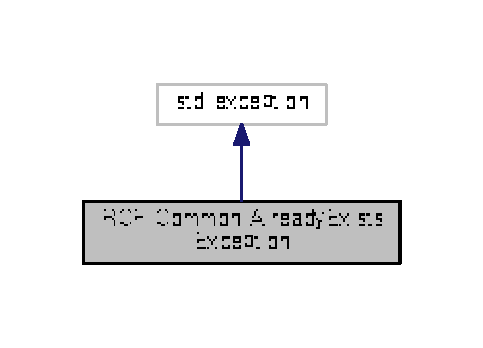
\includegraphics[width=232pt]{class_r_c_f_1_1_common_1_1_already_exists_exception__inherit__graph}
\end{center}
\end{figure}


Collaboration diagram for R\+C\+F\+:\+:Common\+:\+:Already\+Exists\+Exception\+:\nopagebreak
\begin{figure}[H]
\begin{center}
\leavevmode
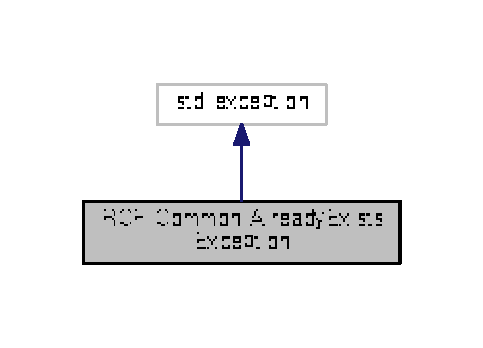
\includegraphics[width=232pt]{class_r_c_f_1_1_common_1_1_already_exists_exception__coll__graph}
\end{center}
\end{figure}
\subsection*{Public Member Functions}
\begin{DoxyCompactItemize}
\item 
\hyperlink{class_r_c_f_1_1_common_1_1_already_exists_exception_a9ba822b6c209ce100cababc81b8a2dcb}{Already\+Exists\+Exception} (std\+::string name, std\+::string error)
\begin{DoxyCompactList}\small\item\em A constructor from query and error. \end{DoxyCompactList}\item 
\hypertarget{class_r_c_f_1_1_common_1_1_already_exists_exception_a6d162fa18122481b50f5994893497838}{}\hyperlink{class_r_c_f_1_1_common_1_1_already_exists_exception_a6d162fa18122481b50f5994893497838}{$\sim$\+Already\+Exists\+Exception} ()  throw ()\label{class_r_c_f_1_1_common_1_1_already_exists_exception_a6d162fa18122481b50f5994893497838}

\begin{DoxyCompactList}\small\item\em A destructor required by std\+::exception. \end{DoxyCompactList}\item 
const char $\ast$ \hyperlink{class_r_c_f_1_1_common_1_1_already_exists_exception_a8bbdb8cc649a303ac9e5547edc0c39e6}{what} () const   throw ()
\begin{DoxyCompactList}\small\item\em A function describing the error. \end{DoxyCompactList}\end{DoxyCompactItemize}


\subsection{Detailed Description}
An exception related to object already existing in given collection. 

\subsection{Constructor \& Destructor Documentation}
\hypertarget{class_r_c_f_1_1_common_1_1_already_exists_exception_a9ba822b6c209ce100cababc81b8a2dcb}{}\index{R\+C\+F\+::\+Common\+::\+Already\+Exists\+Exception@{R\+C\+F\+::\+Common\+::\+Already\+Exists\+Exception}!Already\+Exists\+Exception@{Already\+Exists\+Exception}}
\index{Already\+Exists\+Exception@{Already\+Exists\+Exception}!R\+C\+F\+::\+Common\+::\+Already\+Exists\+Exception@{R\+C\+F\+::\+Common\+::\+Already\+Exists\+Exception}}
\subsubsection[{Already\+Exists\+Exception}]{\setlength{\rightskip}{0pt plus 5cm}R\+C\+F\+::\+Common\+::\+Already\+Exists\+Exception\+::\+Already\+Exists\+Exception (
\begin{DoxyParamCaption}
\item[{std\+::string}]{name, }
\item[{std\+::string}]{error}
\end{DoxyParamCaption}
)}\label{class_r_c_f_1_1_common_1_1_already_exists_exception_a9ba822b6c209ce100cababc81b8a2dcb}


A constructor from query and error. 


\begin{DoxyParams}{Parameters}
{\em name} & Name of an object that already exists. \\
\hline
{\em error} & Additional information. \\
\hline
\end{DoxyParams}


\subsection{Member Function Documentation}
\hypertarget{class_r_c_f_1_1_common_1_1_already_exists_exception_a8bbdb8cc649a303ac9e5547edc0c39e6}{}\index{R\+C\+F\+::\+Common\+::\+Already\+Exists\+Exception@{R\+C\+F\+::\+Common\+::\+Already\+Exists\+Exception}!what@{what}}
\index{what@{what}!R\+C\+F\+::\+Common\+::\+Already\+Exists\+Exception@{R\+C\+F\+::\+Common\+::\+Already\+Exists\+Exception}}
\subsubsection[{what}]{\setlength{\rightskip}{0pt plus 5cm}const char$\ast$ R\+C\+F\+::\+Common\+::\+Already\+Exists\+Exception\+::what (
\begin{DoxyParamCaption}
{}
\end{DoxyParamCaption}
) const throw  ) }\label{class_r_c_f_1_1_common_1_1_already_exists_exception_a8bbdb8cc649a303ac9e5547edc0c39e6}


A function describing the error. 

\begin{DoxyReturn}{Returns}
What has happened. 
\end{DoxyReturn}


The documentation for this class was generated from the following file\+:\begin{DoxyCompactItemize}
\item 
include/\hyperlink{_exceptions_8h}{Exceptions.\+h}\end{DoxyCompactItemize}

\hypertarget{class_r_c_f_1_1_common_1_1_at_end_exception}{}\section{R\+C\+F\+:\+:Common\+:\+:At\+End\+Exception Class Reference}
\label{class_r_c_f_1_1_common_1_1_at_end_exception}\index{R\+C\+F\+::\+Common\+::\+At\+End\+Exception@{R\+C\+F\+::\+Common\+::\+At\+End\+Exception}}


An exception related to iterator being at the end of the collection.  




{\ttfamily \#include $<$Exceptions.\+h$>$}



Inheritance diagram for R\+C\+F\+:\+:Common\+:\+:At\+End\+Exception\+:\nopagebreak
\begin{figure}[H]
\begin{center}
\leavevmode
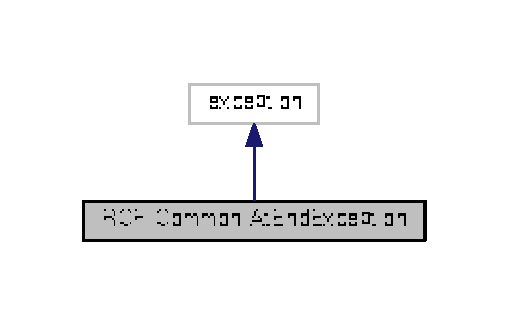
\includegraphics[width=244pt]{class_r_c_f_1_1_common_1_1_at_end_exception__inherit__graph}
\end{center}
\end{figure}


Collaboration diagram for R\+C\+F\+:\+:Common\+:\+:At\+End\+Exception\+:\nopagebreak
\begin{figure}[H]
\begin{center}
\leavevmode
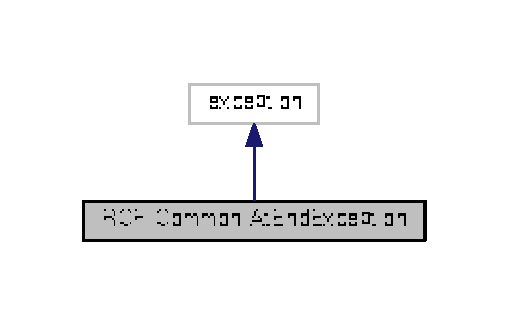
\includegraphics[width=244pt]{class_r_c_f_1_1_common_1_1_at_end_exception__coll__graph}
\end{center}
\end{figure}
\subsection*{Public Member Functions}
\begin{DoxyCompactItemize}
\item 
\hyperlink{class_r_c_f_1_1_common_1_1_at_end_exception_a25e3c7bebad9685dd1ed7f186a0ee5fb}{At\+End\+Exception} (std\+::string error)
\begin{DoxyCompactList}\small\item\em A constructor from error. \end{DoxyCompactList}\item 
\hypertarget{class_r_c_f_1_1_common_1_1_at_end_exception_a6fe2fb26f7d5371d9966b1cdde8162b0}{}\hyperlink{class_r_c_f_1_1_common_1_1_at_end_exception_a6fe2fb26f7d5371d9966b1cdde8162b0}{$\sim$\+At\+End\+Exception} ()  throw ()\label{class_r_c_f_1_1_common_1_1_at_end_exception_a6fe2fb26f7d5371d9966b1cdde8162b0}

\begin{DoxyCompactList}\small\item\em A destructor required by std\+::exception. \end{DoxyCompactList}\item 
const char $\ast$ \hyperlink{class_r_c_f_1_1_common_1_1_at_end_exception_ad7360ef3646bb6bc9bfb18d3f044fd9a}{what} () const   throw ()
\begin{DoxyCompactList}\small\item\em A function describing the error. \end{DoxyCompactList}\end{DoxyCompactItemize}


\subsection{Detailed Description}
An exception related to iterator being at the end of the collection. 

\subsection{Constructor \& Destructor Documentation}
\hypertarget{class_r_c_f_1_1_common_1_1_at_end_exception_a25e3c7bebad9685dd1ed7f186a0ee5fb}{}\index{R\+C\+F\+::\+Common\+::\+At\+End\+Exception@{R\+C\+F\+::\+Common\+::\+At\+End\+Exception}!At\+End\+Exception@{At\+End\+Exception}}
\index{At\+End\+Exception@{At\+End\+Exception}!R\+C\+F\+::\+Common\+::\+At\+End\+Exception@{R\+C\+F\+::\+Common\+::\+At\+End\+Exception}}
\subsubsection[{At\+End\+Exception}]{\setlength{\rightskip}{0pt plus 5cm}R\+C\+F\+::\+Common\+::\+At\+End\+Exception\+::\+At\+End\+Exception (
\begin{DoxyParamCaption}
\item[{std\+::string}]{error}
\end{DoxyParamCaption}
)}\label{class_r_c_f_1_1_common_1_1_at_end_exception_a25e3c7bebad9685dd1ed7f186a0ee5fb}


A constructor from error. 


\begin{DoxyParams}{Parameters}
{\em error} & What has happened. \\
\hline
\end{DoxyParams}


\subsection{Member Function Documentation}
\hypertarget{class_r_c_f_1_1_common_1_1_at_end_exception_ad7360ef3646bb6bc9bfb18d3f044fd9a}{}\index{R\+C\+F\+::\+Common\+::\+At\+End\+Exception@{R\+C\+F\+::\+Common\+::\+At\+End\+Exception}!what@{what}}
\index{what@{what}!R\+C\+F\+::\+Common\+::\+At\+End\+Exception@{R\+C\+F\+::\+Common\+::\+At\+End\+Exception}}
\subsubsection[{what}]{\setlength{\rightskip}{0pt plus 5cm}const char$\ast$ R\+C\+F\+::\+Common\+::\+At\+End\+Exception\+::what (
\begin{DoxyParamCaption}
{}
\end{DoxyParamCaption}
) const throw  ) }\label{class_r_c_f_1_1_common_1_1_at_end_exception_ad7360ef3646bb6bc9bfb18d3f044fd9a}


A function describing the error. 

\begin{DoxyReturn}{Returns}
What has happened. 
\end{DoxyReturn}


The documentation for this class was generated from the following file\+:\begin{DoxyCompactItemize}
\item 
include/\hyperlink{_exceptions_8h}{Exceptions.\+h}\end{DoxyCompactItemize}

\hypertarget{class_r_c_f_1_1_common_1_1_filesystem_exception}{}\section{R\+C\+F\+:\+:Common\+:\+:Filesystem\+Exception Class Reference}
\label{class_r_c_f_1_1_common_1_1_filesystem_exception}\index{R\+C\+F\+::\+Common\+::\+Filesystem\+Exception@{R\+C\+F\+::\+Common\+::\+Filesystem\+Exception}}


An exception related to files and filesystem.  




{\ttfamily \#include $<$Exceptions.\+h$>$}



Inheritance diagram for R\+C\+F\+:\+:Common\+:\+:Filesystem\+Exception\+:\nopagebreak
\begin{figure}[H]
\begin{center}
\leavevmode
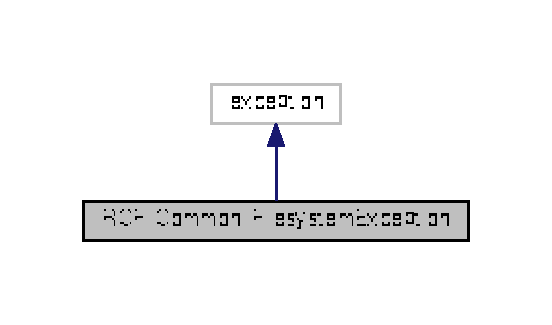
\includegraphics[width=265pt]{class_r_c_f_1_1_common_1_1_filesystem_exception__inherit__graph}
\end{center}
\end{figure}


Collaboration diagram for R\+C\+F\+:\+:Common\+:\+:Filesystem\+Exception\+:\nopagebreak
\begin{figure}[H]
\begin{center}
\leavevmode
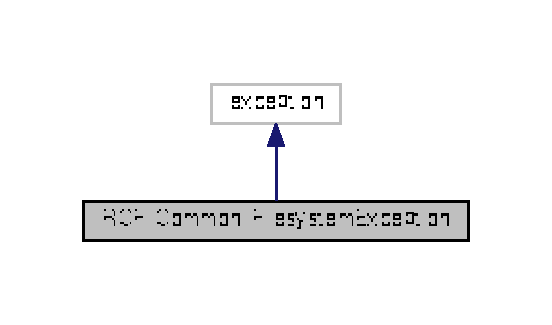
\includegraphics[width=265pt]{class_r_c_f_1_1_common_1_1_filesystem_exception__coll__graph}
\end{center}
\end{figure}
\subsection*{Public Member Functions}
\begin{DoxyCompactItemize}
\item 
\hyperlink{class_r_c_f_1_1_common_1_1_filesystem_exception_adf2e36d11d37710eaea10aebde922f15}{Filesystem\+Exception} (boost\+::filesystem\+::path p, std\+::string error)
\begin{DoxyCompactList}\small\item\em A constructor from path and error. \end{DoxyCompactList}\item 
\hypertarget{class_r_c_f_1_1_common_1_1_filesystem_exception_a0824129ef3ec0388a6d22f797cacfc76}{}\hyperlink{class_r_c_f_1_1_common_1_1_filesystem_exception_a0824129ef3ec0388a6d22f797cacfc76}{$\sim$\+Filesystem\+Exception} ()  throw ()\label{class_r_c_f_1_1_common_1_1_filesystem_exception_a0824129ef3ec0388a6d22f797cacfc76}

\begin{DoxyCompactList}\small\item\em A destructor required by std\+::exception. \end{DoxyCompactList}\item 
const char $\ast$ \hyperlink{class_r_c_f_1_1_common_1_1_filesystem_exception_abec09541bb92502793fa8f9b014792ca}{what} () const   throw ()
\begin{DoxyCompactList}\small\item\em A function describing the error. \end{DoxyCompactList}\end{DoxyCompactItemize}


\subsection{Detailed Description}
An exception related to files and filesystem. 

\subsection{Constructor \& Destructor Documentation}
\hypertarget{class_r_c_f_1_1_common_1_1_filesystem_exception_adf2e36d11d37710eaea10aebde922f15}{}\index{R\+C\+F\+::\+Common\+::\+Filesystem\+Exception@{R\+C\+F\+::\+Common\+::\+Filesystem\+Exception}!Filesystem\+Exception@{Filesystem\+Exception}}
\index{Filesystem\+Exception@{Filesystem\+Exception}!R\+C\+F\+::\+Common\+::\+Filesystem\+Exception@{R\+C\+F\+::\+Common\+::\+Filesystem\+Exception}}
\subsubsection[{Filesystem\+Exception}]{\setlength{\rightskip}{0pt plus 5cm}R\+C\+F\+::\+Common\+::\+Filesystem\+Exception\+::\+Filesystem\+Exception (
\begin{DoxyParamCaption}
\item[{boost\+::filesystem\+::path}]{p, }
\item[{std\+::string}]{error}
\end{DoxyParamCaption}
)}\label{class_r_c_f_1_1_common_1_1_filesystem_exception_adf2e36d11d37710eaea10aebde922f15}


A constructor from path and error. 


\begin{DoxyParams}{Parameters}
{\em p} & A path related to error. \\
\hline
{\em error} & What has happened. \\
\hline
\end{DoxyParams}


\subsection{Member Function Documentation}
\hypertarget{class_r_c_f_1_1_common_1_1_filesystem_exception_abec09541bb92502793fa8f9b014792ca}{}\index{R\+C\+F\+::\+Common\+::\+Filesystem\+Exception@{R\+C\+F\+::\+Common\+::\+Filesystem\+Exception}!what@{what}}
\index{what@{what}!R\+C\+F\+::\+Common\+::\+Filesystem\+Exception@{R\+C\+F\+::\+Common\+::\+Filesystem\+Exception}}
\subsubsection[{what}]{\setlength{\rightskip}{0pt plus 5cm}const char$\ast$ R\+C\+F\+::\+Common\+::\+Filesystem\+Exception\+::what (
\begin{DoxyParamCaption}
{}
\end{DoxyParamCaption}
) const throw  ) }\label{class_r_c_f_1_1_common_1_1_filesystem_exception_abec09541bb92502793fa8f9b014792ca}


A function describing the error. 

\begin{DoxyReturn}{Returns}
What has happened. 
\end{DoxyReturn}


The documentation for this class was generated from the following file\+:\begin{DoxyCompactItemize}
\item 
include/\hyperlink{_exceptions_8h}{Exceptions.\+h}\end{DoxyCompactItemize}

\hypertarget{class_r_c_f_1_1_common_1_1_helper_functions}{}\section{R\+C\+F\+:\+:Common\+:\+:Helper\+Functions Class Reference}
\label{class_r_c_f_1_1_common_1_1_helper_functions}\index{R\+C\+F\+::\+Common\+::\+Helper\+Functions@{R\+C\+F\+::\+Common\+::\+Helper\+Functions}}


A class containing various helper functions for Remote\+Control\+Framework.  




{\ttfamily \#include $<$Helper\+Functions.\+h$>$}

\subsection*{Public Member Functions}
\begin{DoxyCompactItemize}
\item 
std\+::string \hyperlink{class_r_c_f_1_1_common_1_1_helper_functions_a78cc71a8664db194f25e2284f3b2d46a}{get\+Plain\+Home\+Directory} ()
\begin{DoxyCompactList}\small\item\em A function that gets proper home directory cross-\/platform -\/ plain version. \end{DoxyCompactList}\item 
boost\+::filesystem\+::path \hyperlink{class_r_c_f_1_1_common_1_1_helper_functions_aad8b0c0c2e1361e155fd447bde5aa67d}{get\+Home\+Directory} ()
\begin{DoxyCompactList}\small\item\em A function that gets proper home directory cross-\/platform. \end{DoxyCompactList}\item 
void \hyperlink{class_r_c_f_1_1_common_1_1_helper_functions_a35c3890ec6935b09e2dc3ba0a7c111c0}{set\+Input\+Echo} (bool e)
\begin{DoxyCompactList}\small\item\em Multi-\/platform solution for enabling/disabling console input echo for sensitive data entries. \end{DoxyCompactList}\end{DoxyCompactItemize}


\subsection{Detailed Description}
A class containing various helper functions for Remote\+Control\+Framework. 

\subsection{Member Function Documentation}
\hypertarget{class_r_c_f_1_1_common_1_1_helper_functions_aad8b0c0c2e1361e155fd447bde5aa67d}{}\index{R\+C\+F\+::\+Common\+::\+Helper\+Functions@{R\+C\+F\+::\+Common\+::\+Helper\+Functions}!get\+Home\+Directory@{get\+Home\+Directory}}
\index{get\+Home\+Directory@{get\+Home\+Directory}!R\+C\+F\+::\+Common\+::\+Helper\+Functions@{R\+C\+F\+::\+Common\+::\+Helper\+Functions}}
\subsubsection[{get\+Home\+Directory}]{\setlength{\rightskip}{0pt plus 5cm}boost\+::filesystem\+::path R\+C\+F\+::\+Common\+::\+Helper\+Functions\+::get\+Home\+Directory (
\begin{DoxyParamCaption}
{}
\end{DoxyParamCaption}
)}\label{class_r_c_f_1_1_common_1_1_helper_functions_aad8b0c0c2e1361e155fd447bde5aa67d}


A function that gets proper home directory cross-\/platform. 

\begin{DoxyReturn}{Returns}
Detected home directory as boost\+::filesystem\+::path. 
\end{DoxyReturn}
\hypertarget{class_r_c_f_1_1_common_1_1_helper_functions_a78cc71a8664db194f25e2284f3b2d46a}{}\index{R\+C\+F\+::\+Common\+::\+Helper\+Functions@{R\+C\+F\+::\+Common\+::\+Helper\+Functions}!get\+Plain\+Home\+Directory@{get\+Plain\+Home\+Directory}}
\index{get\+Plain\+Home\+Directory@{get\+Plain\+Home\+Directory}!R\+C\+F\+::\+Common\+::\+Helper\+Functions@{R\+C\+F\+::\+Common\+::\+Helper\+Functions}}
\subsubsection[{get\+Plain\+Home\+Directory}]{\setlength{\rightskip}{0pt plus 5cm}std\+::string R\+C\+F\+::\+Common\+::\+Helper\+Functions\+::get\+Plain\+Home\+Directory (
\begin{DoxyParamCaption}
{}
\end{DoxyParamCaption}
)}\label{class_r_c_f_1_1_common_1_1_helper_functions_a78cc71a8664db194f25e2284f3b2d46a}


A function that gets proper home directory cross-\/platform -\/ plain version. 

\begin{DoxyReturn}{Returns}
Detected home directory as std\+::string. 
\end{DoxyReturn}
\hypertarget{class_r_c_f_1_1_common_1_1_helper_functions_a35c3890ec6935b09e2dc3ba0a7c111c0}{}\index{R\+C\+F\+::\+Common\+::\+Helper\+Functions@{R\+C\+F\+::\+Common\+::\+Helper\+Functions}!set\+Input\+Echo@{set\+Input\+Echo}}
\index{set\+Input\+Echo@{set\+Input\+Echo}!R\+C\+F\+::\+Common\+::\+Helper\+Functions@{R\+C\+F\+::\+Common\+::\+Helper\+Functions}}
\subsubsection[{set\+Input\+Echo}]{\setlength{\rightskip}{0pt plus 5cm}void R\+C\+F\+::\+Common\+::\+Helper\+Functions\+::set\+Input\+Echo (
\begin{DoxyParamCaption}
\item[{bool}]{e}
\end{DoxyParamCaption}
)}\label{class_r_c_f_1_1_common_1_1_helper_functions_a35c3890ec6935b09e2dc3ba0a7c111c0}


Multi-\/platform solution for enabling/disabling console input echo for sensitive data entries. 


\begin{DoxyParams}{Parameters}
{\em e} & If echo should be enabled. \\
\hline
\end{DoxyParams}


The documentation for this class was generated from the following file\+:\begin{DoxyCompactItemize}
\item 
include/\hyperlink{_helper_functions_8h}{Helper\+Functions.\+h}\end{DoxyCompactItemize}

\hypertarget{class_r_c_f_1_1_common_1_1_invalid_object_exception}{}\section{R\+C\+F\+:\+:Common\+:\+:Invalid\+Object\+Exception Class Reference}
\label{class_r_c_f_1_1_common_1_1_invalid_object_exception}\index{R\+C\+F\+::\+Common\+::\+Invalid\+Object\+Exception@{R\+C\+F\+::\+Common\+::\+Invalid\+Object\+Exception}}


An exception related to invalidity of object for given action.  




{\ttfamily \#include $<$Exceptions.\+h$>$}



Inheritance diagram for R\+C\+F\+:\+:Common\+:\+:Invalid\+Object\+Exception\+:\nopagebreak
\begin{figure}[H]
\begin{center}
\leavevmode
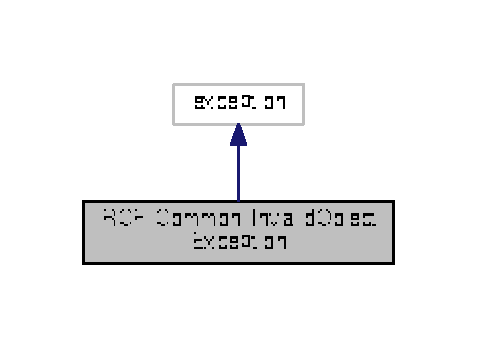
\includegraphics[width=229pt]{class_r_c_f_1_1_common_1_1_invalid_object_exception__inherit__graph}
\end{center}
\end{figure}


Collaboration diagram for R\+C\+F\+:\+:Common\+:\+:Invalid\+Object\+Exception\+:\nopagebreak
\begin{figure}[H]
\begin{center}
\leavevmode
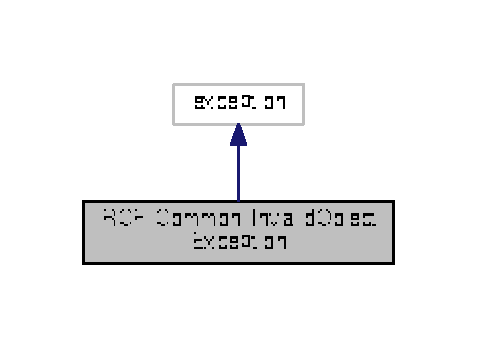
\includegraphics[width=229pt]{class_r_c_f_1_1_common_1_1_invalid_object_exception__coll__graph}
\end{center}
\end{figure}
\subsection*{Public Member Functions}
\begin{DoxyCompactItemize}
\item 
\hyperlink{class_r_c_f_1_1_common_1_1_invalid_object_exception_a3df9541e454574a3d5e6ecc4f90421e9}{Invalid\+Object\+Exception} (std\+::string error)
\begin{DoxyCompactList}\small\item\em A constructor from error. \end{DoxyCompactList}\item 
\hypertarget{class_r_c_f_1_1_common_1_1_invalid_object_exception_a061366b76ff482223c728682784c6cac}{}\hyperlink{class_r_c_f_1_1_common_1_1_invalid_object_exception_a061366b76ff482223c728682784c6cac}{$\sim$\+Invalid\+Object\+Exception} ()  throw ()\label{class_r_c_f_1_1_common_1_1_invalid_object_exception_a061366b76ff482223c728682784c6cac}

\begin{DoxyCompactList}\small\item\em A destructor required by std\+::exception. \end{DoxyCompactList}\item 
const char $\ast$ \hyperlink{class_r_c_f_1_1_common_1_1_invalid_object_exception_a9641c4c66f1b08965e126b651e457b7f}{what} () const   throw ()
\begin{DoxyCompactList}\small\item\em A function describing the error. \end{DoxyCompactList}\end{DoxyCompactItemize}


\subsection{Detailed Description}
An exception related to invalidity of object for given action. 

\subsection{Constructor \& Destructor Documentation}
\hypertarget{class_r_c_f_1_1_common_1_1_invalid_object_exception_a3df9541e454574a3d5e6ecc4f90421e9}{}\index{R\+C\+F\+::\+Common\+::\+Invalid\+Object\+Exception@{R\+C\+F\+::\+Common\+::\+Invalid\+Object\+Exception}!Invalid\+Object\+Exception@{Invalid\+Object\+Exception}}
\index{Invalid\+Object\+Exception@{Invalid\+Object\+Exception}!R\+C\+F\+::\+Common\+::\+Invalid\+Object\+Exception@{R\+C\+F\+::\+Common\+::\+Invalid\+Object\+Exception}}
\subsubsection[{Invalid\+Object\+Exception}]{\setlength{\rightskip}{0pt plus 5cm}R\+C\+F\+::\+Common\+::\+Invalid\+Object\+Exception\+::\+Invalid\+Object\+Exception (
\begin{DoxyParamCaption}
\item[{std\+::string}]{error}
\end{DoxyParamCaption}
)}\label{class_r_c_f_1_1_common_1_1_invalid_object_exception_a3df9541e454574a3d5e6ecc4f90421e9}


A constructor from error. 


\begin{DoxyParams}{Parameters}
{\em error} & What has happened. \\
\hline
\end{DoxyParams}


\subsection{Member Function Documentation}
\hypertarget{class_r_c_f_1_1_common_1_1_invalid_object_exception_a9641c4c66f1b08965e126b651e457b7f}{}\index{R\+C\+F\+::\+Common\+::\+Invalid\+Object\+Exception@{R\+C\+F\+::\+Common\+::\+Invalid\+Object\+Exception}!what@{what}}
\index{what@{what}!R\+C\+F\+::\+Common\+::\+Invalid\+Object\+Exception@{R\+C\+F\+::\+Common\+::\+Invalid\+Object\+Exception}}
\subsubsection[{what}]{\setlength{\rightskip}{0pt plus 5cm}const char$\ast$ R\+C\+F\+::\+Common\+::\+Invalid\+Object\+Exception\+::what (
\begin{DoxyParamCaption}
{}
\end{DoxyParamCaption}
) const throw  ) }\label{class_r_c_f_1_1_common_1_1_invalid_object_exception_a9641c4c66f1b08965e126b651e457b7f}


A function describing the error. 

\begin{DoxyReturn}{Returns}
What has happened. 
\end{DoxyReturn}


The documentation for this class was generated from the following file\+:\begin{DoxyCompactItemize}
\item 
include/\hyperlink{_exceptions_8h}{Exceptions.\+h}\end{DoxyCompactItemize}

\hypertarget{class_r_c_f_1_1_common_1_1_m_hash_engine}{}\section{R\+C\+F\+:\+:Common\+:\+:M\+Hash\+Engine Class Reference}
\label{class_r_c_f_1_1_common_1_1_m_hash_engine}\index{R\+C\+F\+::\+Common\+::\+M\+Hash\+Engine@{R\+C\+F\+::\+Common\+::\+M\+Hash\+Engine}}


A class that handles M\+D5 encryption using M\+Hash.  




{\ttfamily \#include $<$M\+Hash\+Engine.\+h$>$}

\subsection*{Public Member Functions}
\begin{DoxyCompactItemize}
\item 
\hypertarget{class_r_c_f_1_1_common_1_1_m_hash_engine_a47bfc0f8bea510d18d77a3fcbbc02af2}{}\hyperlink{class_r_c_f_1_1_common_1_1_m_hash_engine_a47bfc0f8bea510d18d77a3fcbbc02af2}{M\+Hash\+Engine} ()\label{class_r_c_f_1_1_common_1_1_m_hash_engine_a47bfc0f8bea510d18d77a3fcbbc02af2}

\begin{DoxyCompactList}\small\item\em A constructor initializing M\+Hash. \end{DoxyCompactList}\item 
\hypertarget{class_r_c_f_1_1_common_1_1_m_hash_engine_a38ee073d45a4fc0b70c357964cbf21ff}{}\hyperlink{class_r_c_f_1_1_common_1_1_m_hash_engine_a38ee073d45a4fc0b70c357964cbf21ff}{$\sim$\+M\+Hash\+Engine} ()\label{class_r_c_f_1_1_common_1_1_m_hash_engine_a38ee073d45a4fc0b70c357964cbf21ff}

\begin{DoxyCompactList}\small\item\em A destructor deinitializing M\+Hash. \end{DoxyCompactList}\item 
std\+::string \hyperlink{class_r_c_f_1_1_common_1_1_m_hash_engine_ab2a535745b7b571b156da3b92b8f9346}{get\+Hash} (std\+::string in)
\begin{DoxyCompactList}\small\item\em A function that calculates M\+D5 hash of given string and returns it in hexadecimal form. \end{DoxyCompactList}\end{DoxyCompactItemize}


\subsection{Detailed Description}
A class that handles M\+D5 encryption using M\+Hash. 

\subsection{Member Function Documentation}
\hypertarget{class_r_c_f_1_1_common_1_1_m_hash_engine_ab2a535745b7b571b156da3b92b8f9346}{}\index{R\+C\+F\+::\+Common\+::\+M\+Hash\+Engine@{R\+C\+F\+::\+Common\+::\+M\+Hash\+Engine}!get\+Hash@{get\+Hash}}
\index{get\+Hash@{get\+Hash}!R\+C\+F\+::\+Common\+::\+M\+Hash\+Engine@{R\+C\+F\+::\+Common\+::\+M\+Hash\+Engine}}
\subsubsection[{get\+Hash}]{\setlength{\rightskip}{0pt plus 5cm}std\+::string R\+C\+F\+::\+Common\+::\+M\+Hash\+Engine\+::get\+Hash (
\begin{DoxyParamCaption}
\item[{std\+::string}]{in}
\end{DoxyParamCaption}
)}\label{class_r_c_f_1_1_common_1_1_m_hash_engine_ab2a535745b7b571b156da3b92b8f9346}


A function that calculates M\+D5 hash of given string and returns it in hexadecimal form. 


\begin{DoxyParams}{Parameters}
{\em in} & A string to encrypt \\
\hline
\end{DoxyParams}
\begin{DoxyReturn}{Returns}
A M\+D5 hash of the string in hexadecimal form 
\end{DoxyReturn}


The documentation for this class was generated from the following file\+:\begin{DoxyCompactItemize}
\item 
include/\hyperlink{_m_hash_engine_8h}{M\+Hash\+Engine.\+h}\end{DoxyCompactItemize}

\hypertarget{class_r_c_f_1_1_common_1_1_not_found_exception}{}\section{R\+C\+F\+:\+:Common\+:\+:Not\+Found\+Exception Class Reference}
\label{class_r_c_f_1_1_common_1_1_not_found_exception}\index{R\+C\+F\+::\+Common\+::\+Not\+Found\+Exception@{R\+C\+F\+::\+Common\+::\+Not\+Found\+Exception}}


An exception related to not finding object by given string.  




{\ttfamily \#include $<$Exceptions.\+h$>$}



Inheritance diagram for R\+C\+F\+:\+:Common\+:\+:Not\+Found\+Exception\+:\nopagebreak
\begin{figure}[H]
\begin{center}
\leavevmode
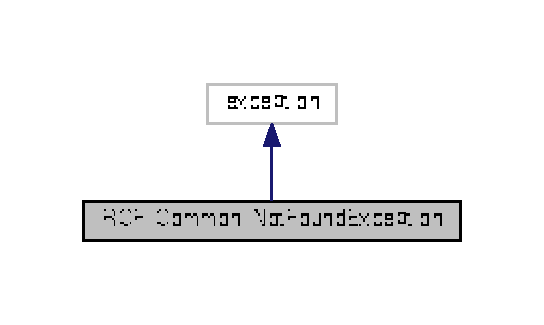
\includegraphics[width=261pt]{class_r_c_f_1_1_common_1_1_not_found_exception__inherit__graph}
\end{center}
\end{figure}


Collaboration diagram for R\+C\+F\+:\+:Common\+:\+:Not\+Found\+Exception\+:\nopagebreak
\begin{figure}[H]
\begin{center}
\leavevmode
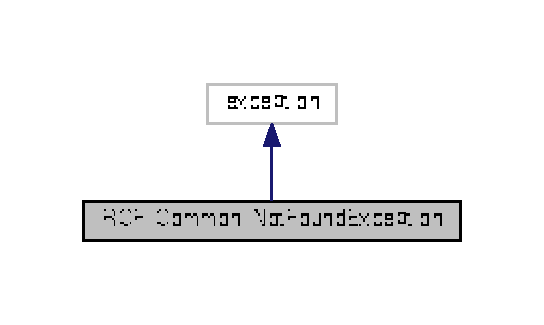
\includegraphics[width=261pt]{class_r_c_f_1_1_common_1_1_not_found_exception__coll__graph}
\end{center}
\end{figure}
\subsection*{Public Member Functions}
\begin{DoxyCompactItemize}
\item 
\hyperlink{class_r_c_f_1_1_common_1_1_not_found_exception_a981160851582a79f993c054a3994af4a}{Not\+Found\+Exception} (std\+::string query, std\+::string error)
\begin{DoxyCompactList}\small\item\em A constructor from query and error. \end{DoxyCompactList}\item 
\hypertarget{class_r_c_f_1_1_common_1_1_not_found_exception_af7699205d30b95939558a55442fd27fd}{}\hyperlink{class_r_c_f_1_1_common_1_1_not_found_exception_af7699205d30b95939558a55442fd27fd}{$\sim$\+Not\+Found\+Exception} ()  throw ()\label{class_r_c_f_1_1_common_1_1_not_found_exception_af7699205d30b95939558a55442fd27fd}

\begin{DoxyCompactList}\small\item\em A destructor required by std\+::exception. \end{DoxyCompactList}\item 
const char $\ast$ \hyperlink{class_r_c_f_1_1_common_1_1_not_found_exception_a1952dae8332c477283bf7193599a6be1}{what} () const   throw ()
\begin{DoxyCompactList}\small\item\em A function describing the error. \end{DoxyCompactList}\end{DoxyCompactItemize}


\subsection{Detailed Description}
An exception related to not finding object by given string. 

\subsection{Constructor \& Destructor Documentation}
\hypertarget{class_r_c_f_1_1_common_1_1_not_found_exception_a981160851582a79f993c054a3994af4a}{}\index{R\+C\+F\+::\+Common\+::\+Not\+Found\+Exception@{R\+C\+F\+::\+Common\+::\+Not\+Found\+Exception}!Not\+Found\+Exception@{Not\+Found\+Exception}}
\index{Not\+Found\+Exception@{Not\+Found\+Exception}!R\+C\+F\+::\+Common\+::\+Not\+Found\+Exception@{R\+C\+F\+::\+Common\+::\+Not\+Found\+Exception}}
\subsubsection[{Not\+Found\+Exception}]{\setlength{\rightskip}{0pt plus 5cm}R\+C\+F\+::\+Common\+::\+Not\+Found\+Exception\+::\+Not\+Found\+Exception (
\begin{DoxyParamCaption}
\item[{std\+::string}]{query, }
\item[{std\+::string}]{error}
\end{DoxyParamCaption}
)}\label{class_r_c_f_1_1_common_1_1_not_found_exception_a981160851582a79f993c054a3994af4a}


A constructor from query and error. 


\begin{DoxyParams}{Parameters}
{\em query} & Query string that was not found. \\
\hline
{\em error} & Additional information. \\
\hline
\end{DoxyParams}


\subsection{Member Function Documentation}
\hypertarget{class_r_c_f_1_1_common_1_1_not_found_exception_a1952dae8332c477283bf7193599a6be1}{}\index{R\+C\+F\+::\+Common\+::\+Not\+Found\+Exception@{R\+C\+F\+::\+Common\+::\+Not\+Found\+Exception}!what@{what}}
\index{what@{what}!R\+C\+F\+::\+Common\+::\+Not\+Found\+Exception@{R\+C\+F\+::\+Common\+::\+Not\+Found\+Exception}}
\subsubsection[{what}]{\setlength{\rightskip}{0pt plus 5cm}const char$\ast$ R\+C\+F\+::\+Common\+::\+Not\+Found\+Exception\+::what (
\begin{DoxyParamCaption}
{}
\end{DoxyParamCaption}
) const throw  ) }\label{class_r_c_f_1_1_common_1_1_not_found_exception_a1952dae8332c477283bf7193599a6be1}


A function describing the error. 

\begin{DoxyReturn}{Returns}
What has happened. 
\end{DoxyReturn}


The documentation for this class was generated from the following file\+:\begin{DoxyCompactItemize}
\item 
include/\hyperlink{_exceptions_8h}{Exceptions.\+h}\end{DoxyCompactItemize}

\hypertarget{class_r_c_f_1_1_common_1_1_parameters_needed_exception}{}\section{R\+C\+F\+:\+:Common\+:\+:Parameters\+Needed\+Exception Class Reference}
\label{class_r_c_f_1_1_common_1_1_parameters_needed_exception}\index{R\+C\+F\+::\+Common\+::\+Parameters\+Needed\+Exception@{R\+C\+F\+::\+Common\+::\+Parameters\+Needed\+Exception}}


An exception related to command needing more parameters.  




{\ttfamily \#include $<$Exceptions.\+h$>$}



Inheritance diagram for R\+C\+F\+:\+:Common\+:\+:Parameters\+Needed\+Exception\+:\nopagebreak
\begin{figure}[H]
\begin{center}
\leavevmode
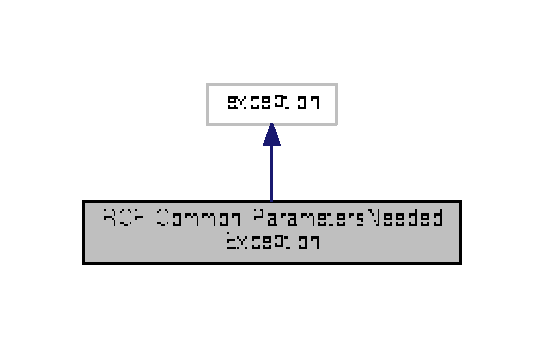
\includegraphics[width=261pt]{class_r_c_f_1_1_common_1_1_parameters_needed_exception__inherit__graph}
\end{center}
\end{figure}


Collaboration diagram for R\+C\+F\+:\+:Common\+:\+:Parameters\+Needed\+Exception\+:\nopagebreak
\begin{figure}[H]
\begin{center}
\leavevmode
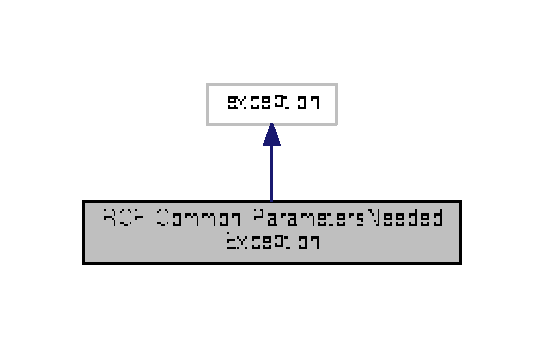
\includegraphics[width=261pt]{class_r_c_f_1_1_common_1_1_parameters_needed_exception__coll__graph}
\end{center}
\end{figure}
\subsection*{Public Member Functions}
\begin{DoxyCompactItemize}
\item 
\hyperlink{class_r_c_f_1_1_common_1_1_parameters_needed_exception_a6d5eb91489f48b7b7749799a2fbb5eb6}{Parameters\+Needed\+Exception} (std\+::string error, int params\+Required, int params\+Given)
\begin{DoxyCompactList}\small\item\em A constructor from params required, params given and error. \end{DoxyCompactList}\item 
\hypertarget{class_r_c_f_1_1_common_1_1_parameters_needed_exception_a20c868291a78bb9775a343f37b21f1d2}{}\hyperlink{class_r_c_f_1_1_common_1_1_parameters_needed_exception_a20c868291a78bb9775a343f37b21f1d2}{$\sim$\+Parameters\+Needed\+Exception} ()  throw ()\label{class_r_c_f_1_1_common_1_1_parameters_needed_exception_a20c868291a78bb9775a343f37b21f1d2}

\begin{DoxyCompactList}\small\item\em A destructor required by std\+::exception. \end{DoxyCompactList}\item 
const char $\ast$ \hyperlink{class_r_c_f_1_1_common_1_1_parameters_needed_exception_a3642a2d5054ca4f1ff3ba76f3c51cf8d}{what} () const   throw ()
\begin{DoxyCompactList}\small\item\em A function describing the error. \end{DoxyCompactList}\end{DoxyCompactItemize}


\subsection{Detailed Description}
An exception related to command needing more parameters. 

\subsection{Constructor \& Destructor Documentation}
\hypertarget{class_r_c_f_1_1_common_1_1_parameters_needed_exception_a6d5eb91489f48b7b7749799a2fbb5eb6}{}\index{R\+C\+F\+::\+Common\+::\+Parameters\+Needed\+Exception@{R\+C\+F\+::\+Common\+::\+Parameters\+Needed\+Exception}!Parameters\+Needed\+Exception@{Parameters\+Needed\+Exception}}
\index{Parameters\+Needed\+Exception@{Parameters\+Needed\+Exception}!R\+C\+F\+::\+Common\+::\+Parameters\+Needed\+Exception@{R\+C\+F\+::\+Common\+::\+Parameters\+Needed\+Exception}}
\subsubsection[{Parameters\+Needed\+Exception}]{\setlength{\rightskip}{0pt plus 5cm}R\+C\+F\+::\+Common\+::\+Parameters\+Needed\+Exception\+::\+Parameters\+Needed\+Exception (
\begin{DoxyParamCaption}
\item[{std\+::string}]{error, }
\item[{int}]{params\+Required, }
\item[{int}]{params\+Given}
\end{DoxyParamCaption}
)}\label{class_r_c_f_1_1_common_1_1_parameters_needed_exception_a6d5eb91489f48b7b7749799a2fbb5eb6}


A constructor from params required, params given and error. 


\begin{DoxyParams}{Parameters}
{\em params\+Required} & A number of parameters that command requires. \\
\hline
{\em params\+Given} & A number of parameters that were given to command. \\
\hline
{\em error} & Additional error information. \\
\hline
\end{DoxyParams}


\subsection{Member Function Documentation}
\hypertarget{class_r_c_f_1_1_common_1_1_parameters_needed_exception_a3642a2d5054ca4f1ff3ba76f3c51cf8d}{}\index{R\+C\+F\+::\+Common\+::\+Parameters\+Needed\+Exception@{R\+C\+F\+::\+Common\+::\+Parameters\+Needed\+Exception}!what@{what}}
\index{what@{what}!R\+C\+F\+::\+Common\+::\+Parameters\+Needed\+Exception@{R\+C\+F\+::\+Common\+::\+Parameters\+Needed\+Exception}}
\subsubsection[{what}]{\setlength{\rightskip}{0pt plus 5cm}const char$\ast$ R\+C\+F\+::\+Common\+::\+Parameters\+Needed\+Exception\+::what (
\begin{DoxyParamCaption}
{}
\end{DoxyParamCaption}
) const throw  ) }\label{class_r_c_f_1_1_common_1_1_parameters_needed_exception_a3642a2d5054ca4f1ff3ba76f3c51cf8d}


A function describing the error. 

\begin{DoxyReturn}{Returns}
What has happened. 
\end{DoxyReturn}


The documentation for this class was generated from the following file\+:\begin{DoxyCompactItemize}
\item 
include/\hyperlink{_exceptions_8h}{Exceptions.\+h}\end{DoxyCompactItemize}

\hypertarget{class_r_c_f_1_1_common_1_1_parser_exception}{}\section{R\+C\+F\+:\+:Common\+:\+:Parser\+Exception Class Reference}
\label{class_r_c_f_1_1_common_1_1_parser_exception}\index{R\+C\+F\+::\+Common\+::\+Parser\+Exception@{R\+C\+F\+::\+Common\+::\+Parser\+Exception}}


An exception related to parsers and formats.  




{\ttfamily \#include $<$Exceptions.\+h$>$}



Inheritance diagram for R\+C\+F\+:\+:Common\+:\+:Parser\+Exception\+:\nopagebreak
\begin{figure}[H]
\begin{center}
\leavevmode
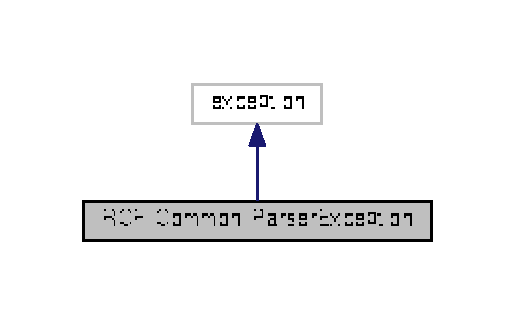
\includegraphics[width=247pt]{class_r_c_f_1_1_common_1_1_parser_exception__inherit__graph}
\end{center}
\end{figure}


Collaboration diagram for R\+C\+F\+:\+:Common\+:\+:Parser\+Exception\+:\nopagebreak
\begin{figure}[H]
\begin{center}
\leavevmode
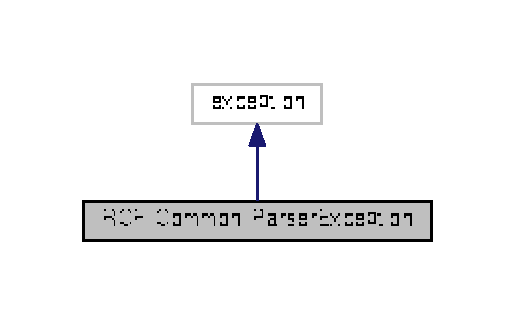
\includegraphics[width=247pt]{class_r_c_f_1_1_common_1_1_parser_exception__coll__graph}
\end{center}
\end{figure}
\subsection*{Public Member Functions}
\begin{DoxyCompactItemize}
\item 
\hyperlink{class_r_c_f_1_1_common_1_1_parser_exception_a5bd15dbf761e09667d86cdd95f980c1b}{Parser\+Exception} (boost\+::filesystem\+::path p, int lineno, std\+::string error)
\begin{DoxyCompactList}\small\item\em A constructor from path, line number and error. \end{DoxyCompactList}\item 
\hypertarget{class_r_c_f_1_1_common_1_1_parser_exception_a99641ad3822bfaa19b4253009fe3c9b3}{}\hyperlink{class_r_c_f_1_1_common_1_1_parser_exception_a99641ad3822bfaa19b4253009fe3c9b3}{$\sim$\+Parser\+Exception} ()  throw ()\label{class_r_c_f_1_1_common_1_1_parser_exception_a99641ad3822bfaa19b4253009fe3c9b3}

\begin{DoxyCompactList}\small\item\em A destructor required by std\+::exception. \end{DoxyCompactList}\item 
const char $\ast$ \hyperlink{class_r_c_f_1_1_common_1_1_parser_exception_a84c7447eaa30971c56fd0cb974095a2a}{what} () const   throw ()
\begin{DoxyCompactList}\small\item\em A function describing the error. \end{DoxyCompactList}\end{DoxyCompactItemize}


\subsection{Detailed Description}
An exception related to parsers and formats. 

\subsection{Constructor \& Destructor Documentation}
\hypertarget{class_r_c_f_1_1_common_1_1_parser_exception_a5bd15dbf761e09667d86cdd95f980c1b}{}\index{R\+C\+F\+::\+Common\+::\+Parser\+Exception@{R\+C\+F\+::\+Common\+::\+Parser\+Exception}!Parser\+Exception@{Parser\+Exception}}
\index{Parser\+Exception@{Parser\+Exception}!R\+C\+F\+::\+Common\+::\+Parser\+Exception@{R\+C\+F\+::\+Common\+::\+Parser\+Exception}}
\subsubsection[{Parser\+Exception}]{\setlength{\rightskip}{0pt plus 5cm}R\+C\+F\+::\+Common\+::\+Parser\+Exception\+::\+Parser\+Exception (
\begin{DoxyParamCaption}
\item[{boost\+::filesystem\+::path}]{p, }
\item[{int}]{lineno, }
\item[{std\+::string}]{error}
\end{DoxyParamCaption}
)}\label{class_r_c_f_1_1_common_1_1_parser_exception_a5bd15dbf761e09667d86cdd95f980c1b}


A constructor from path, line number and error. 


\begin{DoxyParams}{Parameters}
{\em p} & Path of a file related to error. \\
\hline
{\em lineno} & Line number where error in the file is. \\
\hline
{\em error} & What has happened. \\
\hline
\end{DoxyParams}


\subsection{Member Function Documentation}
\hypertarget{class_r_c_f_1_1_common_1_1_parser_exception_a84c7447eaa30971c56fd0cb974095a2a}{}\index{R\+C\+F\+::\+Common\+::\+Parser\+Exception@{R\+C\+F\+::\+Common\+::\+Parser\+Exception}!what@{what}}
\index{what@{what}!R\+C\+F\+::\+Common\+::\+Parser\+Exception@{R\+C\+F\+::\+Common\+::\+Parser\+Exception}}
\subsubsection[{what}]{\setlength{\rightskip}{0pt plus 5cm}const char$\ast$ R\+C\+F\+::\+Common\+::\+Parser\+Exception\+::what (
\begin{DoxyParamCaption}
{}
\end{DoxyParamCaption}
) const throw  ) }\label{class_r_c_f_1_1_common_1_1_parser_exception_a84c7447eaa30971c56fd0cb974095a2a}


A function describing the error. 

\begin{DoxyReturn}{Returns}
What has happened. 
\end{DoxyReturn}


The documentation for this class was generated from the following file\+:\begin{DoxyCompactItemize}
\item 
include/\hyperlink{_exceptions_8h}{Exceptions.\+h}\end{DoxyCompactItemize}

\hypertarget{class_r_c_f_1_1_common_1_1_protocol_exception}{}\section{R\+C\+F\+:\+:Common\+:\+:Protocol\+Exception Class Reference}
\label{class_r_c_f_1_1_common_1_1_protocol_exception}\index{R\+C\+F\+::\+Common\+::\+Protocol\+Exception@{R\+C\+F\+::\+Common\+::\+Protocol\+Exception}}


An exception related to an error during \hyperlink{namespace_r_c_f}{R\+C\+F} Protocol communication.  




{\ttfamily \#include $<$Exceptions.\+h$>$}



Inheritance diagram for R\+C\+F\+:\+:Common\+:\+:Protocol\+Exception\+:\nopagebreak
\begin{figure}[H]
\begin{center}
\leavevmode
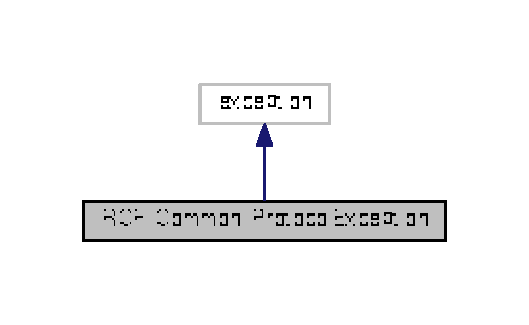
\includegraphics[width=254pt]{class_r_c_f_1_1_common_1_1_protocol_exception__inherit__graph}
\end{center}
\end{figure}


Collaboration diagram for R\+C\+F\+:\+:Common\+:\+:Protocol\+Exception\+:\nopagebreak
\begin{figure}[H]
\begin{center}
\leavevmode
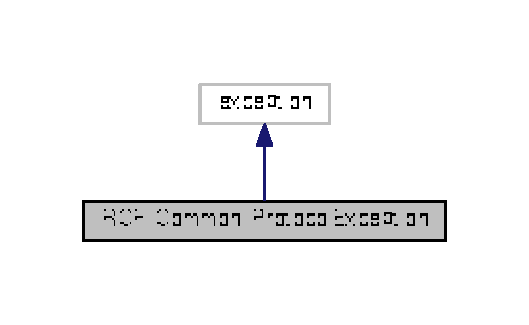
\includegraphics[width=254pt]{class_r_c_f_1_1_common_1_1_protocol_exception__coll__graph}
\end{center}
\end{figure}
\subsection*{Public Member Functions}
\begin{DoxyCompactItemize}
\item 
\hyperlink{class_r_c_f_1_1_common_1_1_protocol_exception_aa32f723d59444c644cb5ed4fe8ceaefc}{Protocol\+Exception} (std\+::string error)
\begin{DoxyCompactList}\small\item\em A constructor from error. \end{DoxyCompactList}\item 
\hypertarget{class_r_c_f_1_1_common_1_1_protocol_exception_a7a3b9c69b7da24d3891c76e7b12508c3}{}\hyperlink{class_r_c_f_1_1_common_1_1_protocol_exception_a7a3b9c69b7da24d3891c76e7b12508c3}{$\sim$\+Protocol\+Exception} ()  throw ()\label{class_r_c_f_1_1_common_1_1_protocol_exception_a7a3b9c69b7da24d3891c76e7b12508c3}

\begin{DoxyCompactList}\small\item\em A destructor required by std\+::exception. \end{DoxyCompactList}\item 
const char $\ast$ \hyperlink{class_r_c_f_1_1_common_1_1_protocol_exception_a2fa21d12baab457ceb141f1c37aa2453}{what} () const   throw ()
\begin{DoxyCompactList}\small\item\em A function describing the error. \end{DoxyCompactList}\end{DoxyCompactItemize}


\subsection{Detailed Description}
An exception related to an error during \hyperlink{namespace_r_c_f}{R\+C\+F} Protocol communication. 

\subsection{Constructor \& Destructor Documentation}
\hypertarget{class_r_c_f_1_1_common_1_1_protocol_exception_aa32f723d59444c644cb5ed4fe8ceaefc}{}\index{R\+C\+F\+::\+Common\+::\+Protocol\+Exception@{R\+C\+F\+::\+Common\+::\+Protocol\+Exception}!Protocol\+Exception@{Protocol\+Exception}}
\index{Protocol\+Exception@{Protocol\+Exception}!R\+C\+F\+::\+Common\+::\+Protocol\+Exception@{R\+C\+F\+::\+Common\+::\+Protocol\+Exception}}
\subsubsection[{Protocol\+Exception}]{\setlength{\rightskip}{0pt plus 5cm}R\+C\+F\+::\+Common\+::\+Protocol\+Exception\+::\+Protocol\+Exception (
\begin{DoxyParamCaption}
\item[{std\+::string}]{error}
\end{DoxyParamCaption}
)}\label{class_r_c_f_1_1_common_1_1_protocol_exception_aa32f723d59444c644cb5ed4fe8ceaefc}


A constructor from error. 


\begin{DoxyParams}{Parameters}
{\em error} & What has happened. \\
\hline
\end{DoxyParams}


\subsection{Member Function Documentation}
\hypertarget{class_r_c_f_1_1_common_1_1_protocol_exception_a2fa21d12baab457ceb141f1c37aa2453}{}\index{R\+C\+F\+::\+Common\+::\+Protocol\+Exception@{R\+C\+F\+::\+Common\+::\+Protocol\+Exception}!what@{what}}
\index{what@{what}!R\+C\+F\+::\+Common\+::\+Protocol\+Exception@{R\+C\+F\+::\+Common\+::\+Protocol\+Exception}}
\subsubsection[{what}]{\setlength{\rightskip}{0pt plus 5cm}const char$\ast$ R\+C\+F\+::\+Common\+::\+Protocol\+Exception\+::what (
\begin{DoxyParamCaption}
{}
\end{DoxyParamCaption}
) const throw  ) }\label{class_r_c_f_1_1_common_1_1_protocol_exception_a2fa21d12baab457ceb141f1c37aa2453}


A function describing the error. 

\begin{DoxyReturn}{Returns}
What has happened. 
\end{DoxyReturn}


The documentation for this class was generated from the following file\+:\begin{DoxyCompactItemize}
\item 
include/\hyperlink{_exceptions_8h}{Exceptions.\+h}\end{DoxyCompactItemize}

\hypertarget{class_r_c_f_1_1_common_1_1_runtime_exception}{}\section{R\+C\+F\+:\+:Common\+:\+:Runtime\+Exception Class Reference}
\label{class_r_c_f_1_1_common_1_1_runtime_exception}\index{R\+C\+F\+::\+Common\+::\+Runtime\+Exception@{R\+C\+F\+::\+Common\+::\+Runtime\+Exception}}


An exception related to error during program execution.  




{\ttfamily \#include $<$Exceptions.\+h$>$}



Inheritance diagram for R\+C\+F\+:\+:Common\+:\+:Runtime\+Exception\+:\nopagebreak
\begin{figure}[H]
\begin{center}
\leavevmode
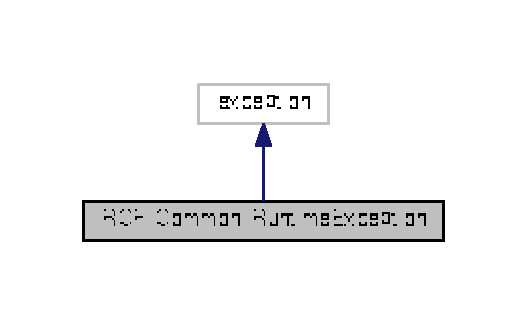
\includegraphics[width=253pt]{class_r_c_f_1_1_common_1_1_runtime_exception__inherit__graph}
\end{center}
\end{figure}


Collaboration diagram for R\+C\+F\+:\+:Common\+:\+:Runtime\+Exception\+:\nopagebreak
\begin{figure}[H]
\begin{center}
\leavevmode
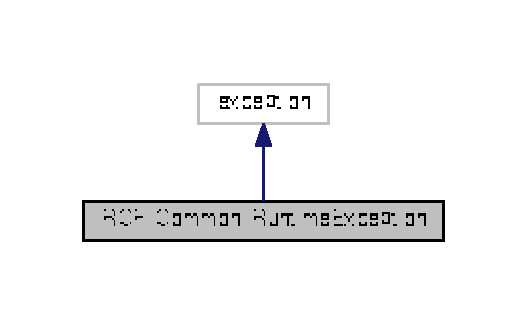
\includegraphics[width=253pt]{class_r_c_f_1_1_common_1_1_runtime_exception__coll__graph}
\end{center}
\end{figure}
\subsection*{Public Member Functions}
\begin{DoxyCompactItemize}
\item 
\hyperlink{class_r_c_f_1_1_common_1_1_runtime_exception_a71a5d289813b628b06d996331fe43896}{Runtime\+Exception} (std\+::string error)
\begin{DoxyCompactList}\small\item\em A constructor from error. \end{DoxyCompactList}\item 
\hypertarget{class_r_c_f_1_1_common_1_1_runtime_exception_aedbe6d21c73d6a74b42deccf5f189de9}{}\hyperlink{class_r_c_f_1_1_common_1_1_runtime_exception_aedbe6d21c73d6a74b42deccf5f189de9}{$\sim$\+Runtime\+Exception} ()  throw ()\label{class_r_c_f_1_1_common_1_1_runtime_exception_aedbe6d21c73d6a74b42deccf5f189de9}

\begin{DoxyCompactList}\small\item\em A destructor required by std\+::exception. \end{DoxyCompactList}\item 
const char $\ast$ \hyperlink{class_r_c_f_1_1_common_1_1_runtime_exception_a49c8baaf5354898bf9780de191a6275c}{what} () const   throw ()
\begin{DoxyCompactList}\small\item\em A function describing the error. \end{DoxyCompactList}\end{DoxyCompactItemize}


\subsection{Detailed Description}
An exception related to error during program execution. 

\subsection{Constructor \& Destructor Documentation}
\hypertarget{class_r_c_f_1_1_common_1_1_runtime_exception_a71a5d289813b628b06d996331fe43896}{}\index{R\+C\+F\+::\+Common\+::\+Runtime\+Exception@{R\+C\+F\+::\+Common\+::\+Runtime\+Exception}!Runtime\+Exception@{Runtime\+Exception}}
\index{Runtime\+Exception@{Runtime\+Exception}!R\+C\+F\+::\+Common\+::\+Runtime\+Exception@{R\+C\+F\+::\+Common\+::\+Runtime\+Exception}}
\subsubsection[{Runtime\+Exception}]{\setlength{\rightskip}{0pt plus 5cm}R\+C\+F\+::\+Common\+::\+Runtime\+Exception\+::\+Runtime\+Exception (
\begin{DoxyParamCaption}
\item[{std\+::string}]{error}
\end{DoxyParamCaption}
)}\label{class_r_c_f_1_1_common_1_1_runtime_exception_a71a5d289813b628b06d996331fe43896}


A constructor from error. 


\begin{DoxyParams}{Parameters}
{\em error} & What has happened. \\
\hline
\end{DoxyParams}


\subsection{Member Function Documentation}
\hypertarget{class_r_c_f_1_1_common_1_1_runtime_exception_a49c8baaf5354898bf9780de191a6275c}{}\index{R\+C\+F\+::\+Common\+::\+Runtime\+Exception@{R\+C\+F\+::\+Common\+::\+Runtime\+Exception}!what@{what}}
\index{what@{what}!R\+C\+F\+::\+Common\+::\+Runtime\+Exception@{R\+C\+F\+::\+Common\+::\+Runtime\+Exception}}
\subsubsection[{what}]{\setlength{\rightskip}{0pt plus 5cm}const char$\ast$ R\+C\+F\+::\+Common\+::\+Runtime\+Exception\+::what (
\begin{DoxyParamCaption}
{}
\end{DoxyParamCaption}
) const throw  ) }\label{class_r_c_f_1_1_common_1_1_runtime_exception_a49c8baaf5354898bf9780de191a6275c}


A function describing the error. 

\begin{DoxyReturn}{Returns}
What has happened. 
\end{DoxyReturn}


The documentation for this class was generated from the following file\+:\begin{DoxyCompactItemize}
\item 
include/\hyperlink{_exceptions_8h}{Exceptions.\+h}\end{DoxyCompactItemize}

\chapter{File Documentation}
\hypertarget{_exceptions_8h}{}\section{include/\+Exceptions.h File Reference}
\label{_exceptions_8h}\index{include/\+Exceptions.\+h@{include/\+Exceptions.\+h}}


Common exceptions for Remote\+Control\+Framework.  


{\ttfamily \#include $<$exception$>$}\\*
{\ttfamily \#include $<$string$>$}\\*
{\ttfamily \#include $<$boost/filesystem.\+hpp$>$}\\*
Include dependency graph for Exceptions.\+h\+:\nopagebreak
\begin{figure}[H]
\begin{center}
\leavevmode
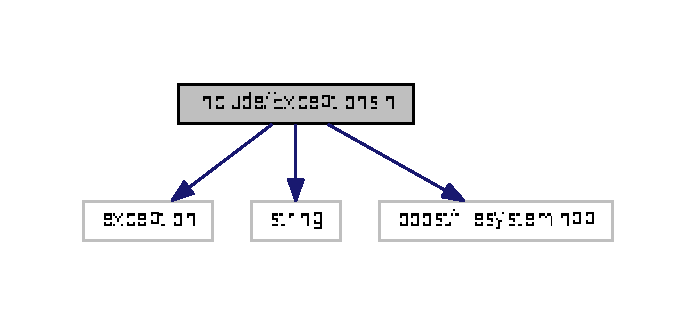
\includegraphics[width=334pt]{_exceptions_8h__incl}
\end{center}
\end{figure}
This graph shows which files directly or indirectly include this file\+:\nopagebreak
\begin{figure}[H]
\begin{center}
\leavevmode
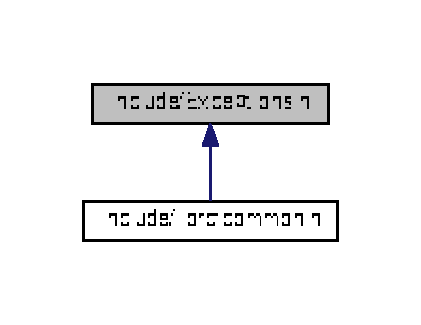
\includegraphics[width=202pt]{_exceptions_8h__dep__incl}
\end{center}
\end{figure}
\subsection*{Classes}
\begin{DoxyCompactItemize}
\item 
class \hyperlink{class_r_c_f_1_1_common_1_1_filesystem_exception}{R\+C\+F\+::\+Common\+::\+Filesystem\+Exception}
\begin{DoxyCompactList}\small\item\em An exception related to files and filesystem. \end{DoxyCompactList}\item 
class \hyperlink{class_r_c_f_1_1_common_1_1_invalid_object_exception}{R\+C\+F\+::\+Common\+::\+Invalid\+Object\+Exception}
\begin{DoxyCompactList}\small\item\em An exception related to invalidity of object for given action. \end{DoxyCompactList}\item 
class \hyperlink{class_r_c_f_1_1_common_1_1_parser_exception}{R\+C\+F\+::\+Common\+::\+Parser\+Exception}
\begin{DoxyCompactList}\small\item\em An exception related to parsers and formats. \end{DoxyCompactList}\item 
class \hyperlink{class_r_c_f_1_1_common_1_1_not_found_exception}{R\+C\+F\+::\+Common\+::\+Not\+Found\+Exception}
\begin{DoxyCompactList}\small\item\em An exception related to not finding object by given string. \end{DoxyCompactList}\item 
class \hyperlink{class_r_c_f_1_1_common_1_1_already_exists_exception}{R\+C\+F\+::\+Common\+::\+Already\+Exists\+Exception}
\begin{DoxyCompactList}\small\item\em An exception related to object already existing in given collection. \end{DoxyCompactList}\item 
class \hyperlink{class_r_c_f_1_1_common_1_1_at_end_exception}{R\+C\+F\+::\+Common\+::\+At\+End\+Exception}
\begin{DoxyCompactList}\small\item\em An exception related to iterator being at the end of the collection. \end{DoxyCompactList}\item 
class \hyperlink{class_r_c_f_1_1_common_1_1_parameters_needed_exception}{R\+C\+F\+::\+Common\+::\+Parameters\+Needed\+Exception}
\begin{DoxyCompactList}\small\item\em An exception related to command needing more parameters. \end{DoxyCompactList}\item 
class \hyperlink{class_r_c_f_1_1_common_1_1_runtime_exception}{R\+C\+F\+::\+Common\+::\+Runtime\+Exception}
\begin{DoxyCompactList}\small\item\em An exception related to error during program execution. \end{DoxyCompactList}\item 
class \hyperlink{class_r_c_f_1_1_common_1_1_protocol_exception}{R\+C\+F\+::\+Common\+::\+Protocol\+Exception}
\begin{DoxyCompactList}\small\item\em An exception related to an error during \hyperlink{namespace_r_c_f}{R\+C\+F} Protocol communication. \end{DoxyCompactList}\end{DoxyCompactItemize}
\subsection*{Namespaces}
\begin{DoxyCompactItemize}
\item 
 \hyperlink{namespace_r_c_f}{R\+C\+F}
\begin{DoxyCompactList}\small\item\em A global namespace for Remote\+Control\+Framework. \end{DoxyCompactList}\item 
 \hyperlink{namespace_r_c_f_1_1_common}{R\+C\+F\+::\+Common}
\begin{DoxyCompactList}\small\item\em A namespace for common Remote\+Control\+Framework classes. \end{DoxyCompactList}\end{DoxyCompactItemize}


\subsection{Detailed Description}
Common exceptions for Remote\+Control\+Framework. 

\begin{DoxyAuthor}{Author}
Phitherek\+\_\+ 
\end{DoxyAuthor}
\begin{DoxyDate}{Date}
2014 
\end{DoxyDate}
\begin{DoxyVersion}{Version}
0.\+1 
\end{DoxyVersion}

\hypertarget{_helper_functions_8h}{}\section{include/\+Helper\+Functions.h File Reference}
\label{_helper_functions_8h}\index{include/\+Helper\+Functions.\+h@{include/\+Helper\+Functions.\+h}}


Various helper functions for Remote\+Control\+Framework.  


{\ttfamily \#include $<$string$>$}\\*
{\ttfamily \#include $<$boost/filesystem.\+hpp$>$}\\*
{\ttfamily \#include $<$boost/predef.\+h$>$}\\*
Include dependency graph for Helper\+Functions.\+h\+:\nopagebreak
\begin{figure}[H]
\begin{center}
\leavevmode
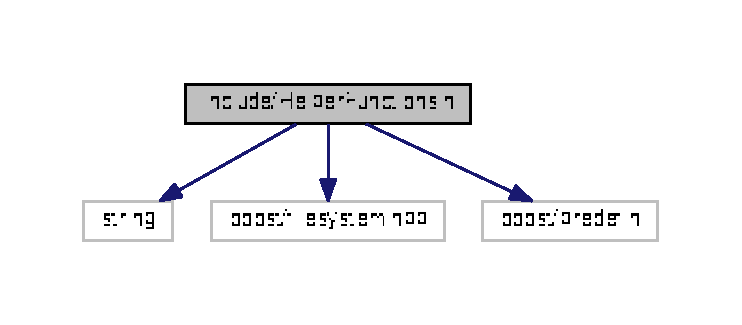
\includegraphics[width=350pt]{_helper_functions_8h__incl}
\end{center}
\end{figure}
This graph shows which files directly or indirectly include this file\+:\nopagebreak
\begin{figure}[H]
\begin{center}
\leavevmode
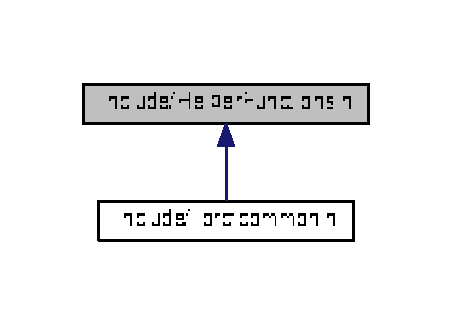
\includegraphics[width=217pt]{_helper_functions_8h__dep__incl}
\end{center}
\end{figure}
\subsection*{Classes}
\begin{DoxyCompactItemize}
\item 
class \hyperlink{class_r_c_f_1_1_common_1_1_helper_functions}{R\+C\+F\+::\+Common\+::\+Helper\+Functions}
\begin{DoxyCompactList}\small\item\em A class containing various helper functions for Remote\+Control\+Framework. \end{DoxyCompactList}\end{DoxyCompactItemize}
\subsection*{Namespaces}
\begin{DoxyCompactItemize}
\item 
 \hyperlink{namespace_r_c_f}{R\+C\+F}
\begin{DoxyCompactList}\small\item\em A global namespace for Remote\+Control\+Framework. \end{DoxyCompactList}\item 
 \hyperlink{namespace_r_c_f_1_1_common}{R\+C\+F\+::\+Common}
\begin{DoxyCompactList}\small\item\em A namespace for common Remote\+Control\+Framework classes. \end{DoxyCompactList}\end{DoxyCompactItemize}


\subsection{Detailed Description}
Various helper functions for Remote\+Control\+Framework. 

\begin{DoxyAuthor}{Author}
Phitherek\+\_\+ 
\end{DoxyAuthor}
\begin{DoxyDate}{Date}
2014-\/2015 
\end{DoxyDate}
\begin{DoxyVersion}{Version}
0.\+1 
\end{DoxyVersion}

\hypertarget{_m_hash_engine_8h}{}\section{include/\+M\+Hash\+Engine.h File Reference}
\label{_m_hash_engine_8h}\index{include/\+M\+Hash\+Engine.\+h@{include/\+M\+Hash\+Engine.\+h}}


A class that handles M\+D5 encryption using M\+Hash library (compile with -\/lmhash)  


{\ttfamily \#include \char`\"{}mhash.\+h\char`\"{}}\\*
{\ttfamily \#include $<$string$>$}\\*
Include dependency graph for M\+Hash\+Engine.\+h\+:\nopagebreak
\begin{figure}[H]
\begin{center}
\leavevmode
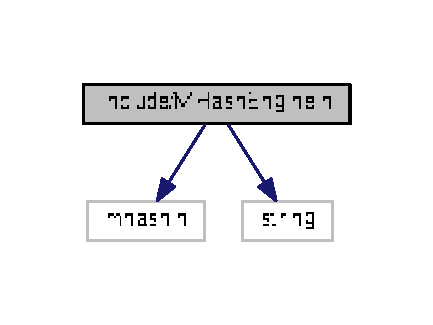
\includegraphics[width=208pt]{_m_hash_engine_8h__incl}
\end{center}
\end{figure}
This graph shows which files directly or indirectly include this file\+:\nopagebreak
\begin{figure}[H]
\begin{center}
\leavevmode
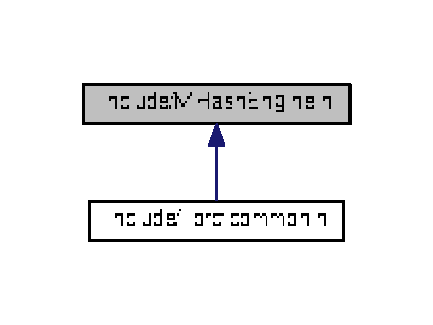
\includegraphics[width=208pt]{_m_hash_engine_8h__dep__incl}
\end{center}
\end{figure}
\subsection*{Classes}
\begin{DoxyCompactItemize}
\item 
class \hyperlink{class_r_c_f_1_1_common_1_1_m_hash_engine}{R\+C\+F\+::\+Common\+::\+M\+Hash\+Engine}
\begin{DoxyCompactList}\small\item\em A class that handles M\+D5 encryption using M\+Hash. \end{DoxyCompactList}\end{DoxyCompactItemize}
\subsection*{Namespaces}
\begin{DoxyCompactItemize}
\item 
 \hyperlink{namespace_r_c_f}{R\+C\+F}
\begin{DoxyCompactList}\small\item\em A global namespace for Remote\+Control\+Framework. \end{DoxyCompactList}\item 
 \hyperlink{namespace_r_c_f_1_1_common}{R\+C\+F\+::\+Common}
\begin{DoxyCompactList}\small\item\em A namespace for common Remote\+Control\+Framework classes. \end{DoxyCompactList}\end{DoxyCompactItemize}


\subsection{Detailed Description}
A class that handles M\+D5 encryption using M\+Hash library (compile with -\/lmhash) 

\begin{DoxyAuthor}{Author}
Phitherek\+\_\+ 
\end{DoxyAuthor}
\begin{DoxyDate}{Date}
2014 
\end{DoxyDate}
\begin{DoxyVersion}{Version}
0.\+1 
\end{DoxyVersion}

%--- End generated contents ---

% Index
\backmatter
\newpage
\phantomsection
\clearemptydoublepage
\addcontentsline{toc}{chapter}{Index}
\printindex

\end{document}
